\documentclass[tikz,border=5pt]{standalone}
\begin{document}
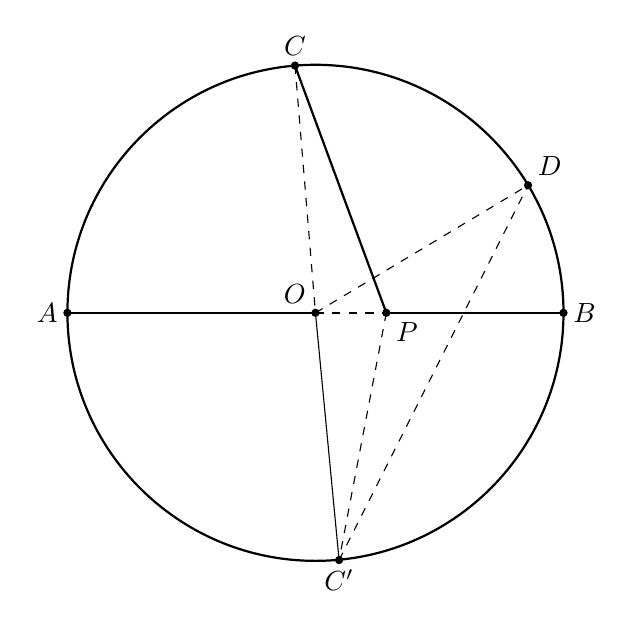
\begin{tikzpicture}
  % 坐标
  \coordinate (O)  at (0,0);
  \coordinate (A)  at (-3.15,0);
  \coordinate (B)  at (3.15,0);
  \coordinate (C)  at (-0.26,3.14);
  \coordinate (Cp) at (0.30,-3.14);
  \coordinate (D)  at (2.70,1.62);
  \coordinate (P)  at (0.90,0);

  % 圆
  \draw[thick] (O) circle (3.15);

  % 直径 AB：AO 实线，OP 虚线，PB 实线
  \draw[thick] (A) -- (O);
  \draw[thick, dashed] (O) -- (P);
  \draw[thick] (P) -- (B);

  % 其余线段
  \draw[thick] (C) -- (P);
  \draw[dashed] (C) -- (O);
  \draw (O) -- (Cp);
  \draw[dashed] (O) -- (D);
  \draw[dashed] (P) -- (Cp);
  \draw[dashed] (Cp) -- (D);

  % 点
  \foreach \p in {A,B,C,Cp,D,O,P}
    \fill (\p) circle (1.5pt);

  % 标签
  \node[left]        at (A)  {$A$};
  \node[right]       at (B)  {$B$};
  \node[above]       at (C)  {$C$};
  \node[below]       at (Cp) {$C'$};
  \node[above right] at (D)  {$D$};
  \node[above left]  at (O)  {$O$};
  \node[below right] at (P)  {$P$};
\end{tikzpicture}
\end{document}
